%! Licence = CC BY-NC-SA 4.0

%! Author = gianfluetsch
%! Date = 30. Dez 2021
%! Project = cydef_summary

\section{MISP}
MISP Threat Sharing (MISP) is an open source threat intelligence platform. The project develops utilities and documentation for more effective threat intelligence, by sharing indicators of compromise.

\subsection{Introduction}

\subsubsection{MISP Usage}
MISP is used for collecting and categorizing malware samples. These events can then be shared und used for other communities.

\subsubsection{Feed}
The feeds can be used as a source of correlations for all of your events and attributes without the need to import them directly into your system. The MISP feed system allows for fast correlation but also a for quick comparisons of the feeds against one another.

\subsection{Phishing Email}

\subsubsection{Difference Attributes \& Objects in an event}
An attribute is a single value stored in MISP with a specific category. An object in opposite, is like a collection of attributes, which are related together (for example: Person - first name and last name are together an object, if they are not linked, then they are attributes)

\subsubsection{Why are you just able to merge to person object and not to a employee object?}
There aren't enough parameter provided for MISP in order to merge to an employee object.

\subsubsection{Why does the IP address not show up as a correlation between the two events?}
The sender email address is the same, but google sent the mail from different mailserver, so the ip address is different. That means, that MISP isn't able to correlate them by the IP address.

\subsection{Malware Sandbox}

\subsubsection{Describe the advantages \& disadvantages of uploading the file directly to MISP vs. uploading the file to a sandbox}
Malware samples are dangerous. Therefore we can use Sandboxes to see what effect certain malicious files have on a certain system and if they do any harm. Advantages to uploading the Malware to a online sandbox (like Hybrid-Analysis) are that they gather information about the file(s) from different sources (virus total etc.) and they are accessible from a browser. This makes it very convenient to test malicious files.
On the other hand, a file can be uploaded directly to MISP. The instance then created a set of hashes of that file which can lead to correlation of other events later. This makes it useful to identify if the file already has appeared elsewhere.
In the end, a combination of using a online malware sandbox and MIPS's internal tools is the best option.

\subsubsection{Please examine the following correlation graph. Describe what you can interpret from the given data}
\begin{center}
    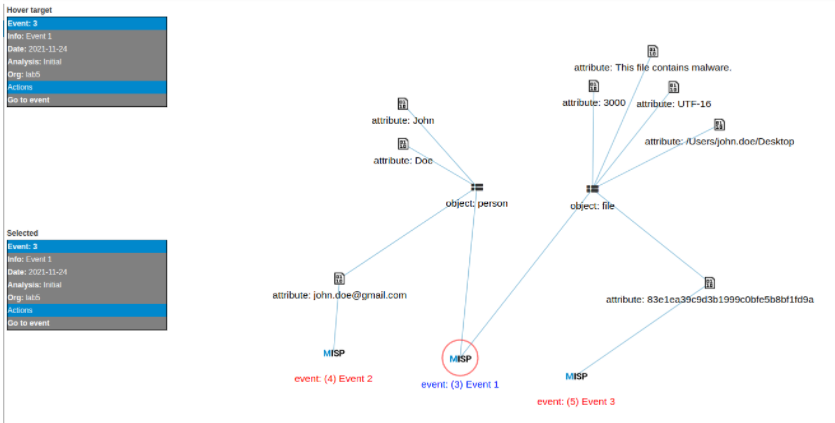
\includegraphics[width=1.0\linewidth]{misp_sandbox}
    \vspace{-8pt}
\end{center}

The graph shows three events that correlate in some way with each other. We are currently looking from Event 1's point of view. Event 2 has a connection to the attribute john.doe@gmail.com which connects to Event 1. Event 1 then has connection to Event 3 over a file hash.
The graph also shows other attributes of the file object and person object, like first name, last name, file size, file path and so on.
The graph gives a quick overview of how the attributes correlate. To go further in detail, the events can be viewed individually.

\subsection{API}

\subsubsection{Describe what you can do with the MISP API and who might use this API}
MISP can and will be used in combination with other tools. For example a firewall might needs access to certain parts of information that MISP collects. This could be a feed of bad IPs, that MISP collects and the firewall then enforces rules to prevent access to those IPs.

\subsubsection{Python Script}
PThe following script will return if the event is published, how many attributes the event has and what distribution level it has.

\begin{lstlisting}[language=Python]
    from pymisp import PyMISP

    misp_url = "http://localhost:10000/"
    misp_key = "eFCeKeKFq6BJIVzHrzTUxW7pYoN0hj0Xur9ca0vV"
    misp_verifycert = False

    myMispInstance = PyMISP(misp_url, misp_key, misp_verifycert)
    event = myMispInstance.get_event(6)

    print(f"Event published: {event['Event']['published']}")
    print(f"Attribute Count: {event['Event']['attribute_count']}")
    print(f"Distribution Level: {event['Event']['distribution']}")
\end{lstlisting}



\subsection{Event Graph | MITRE ATT\&CK}

\subsubsection{What are advantages of using the MISP event graph?}
Nobody likes reading through long paragraphs of documentation. Get a little summary by the graphics, how the objects and/or attributes are linked is more userfriedly. And the researcher will save time too!

\subsubsection{What is the difference between tags and galaxies in MISP?}
MISP galaxies are a method used to express a large object (called cluster) that can be attached to MISP events or attributes (way to attach more complex structures to data). There are default vocabularies available in MISP galaxy from existing standards (like STIX, Veris, ATT\&CK, ...) or your MISP site administrator can create custom ones for you.\\

Tag are uses to tag events, objects or attributes (obviously). Tags can be set from Taxonomy or Custom tags. Example for an tag could be "tlp:white"

\subsection{Sharing}

\textcolor{red}{-> Marius, wichtigste Punkte für Sharing}

\subsubsection{On your instance A, you defined the distribution level of this event as Community only, but on instance B the distribution level is set to Organisation - Why?}
The distribution level can vary from instance to instance. The highest level is always at the organisation which created (and owns) the event.

\subsubsection{Why is it NOT necessary to update the distribution level of this event?}
Org F (on the same instance) cannot see the event.

\subsubsection{To which other MISP instances will the MISP instance B forward the Hello World from Org A event?}
The event will be shared to all instances, because the distribution level is set to All communities.

\subsubsection{Difference between the synchronisation philosophy and feeds in MISP?}
Feeds lets you pull data from an URL (external sources) or files. On the other hand synchronisation lets you pull or / and push event between multiple MISP instances.

\subsection{Expansion Modules}

\subsubsection{Why should even foreign (trustworthy) Modules be used?}
They could support you during research. MISP Modules can save you a lot of repetitive work

\subsubsection{Why does MISP introduced a feature like Modules, when it's already open source?}
No one is able to develop a tool that satisfies all users with all their desired features. So MISP invented Modules wich can be used like mods in games.



\subsection{Warning Lists}

\subsubsection{Explain why this information (warning lists) is useful and how investigators might use this feature.}
This information can be very valuable for someone who adds an event. The information that a certain IP address belongs to for example a Google IP range can be a useful hint. The ability to enable and disable the warninglists individually can be useful as well, because not every list is relevant for every organisation.

\subsubsection{Why does the value bit.ly set off two warning?}
This value appears in two lists. It is in the URL Shorteners domain and Office 365 URLs list included.

\subsubsection{Try to add a second attribute to the event and add a value also in one of the enabled warninglists. Does it also show up as a warning?}
As long as the value added is in the correct category and type (and in the warninglist) the attribute warning shows up like this.

\subsection{Cluster vs. Galaxies}
\textcolor{red}{-> Marius}

